\section{Natural Language Processing}
\subsection{Preprocessing}
\subsubsection{Tokenization}
Tokenization is used to split up words or other input data into smaller \textbf{tokens}. This ensures that the inputs are more regular in size and introduces inter-word context.

\subsection{Embeddings}

\subsubsection{Bag of Words}
BoW is a simple way of representing text, by counting the number of occurences of the $n-1$ most frequent words (all other words are assigned `UNK').
This results in a $n$ dimensional vector representation of the text sequence.
\subsubsection{Word Embeddings}
In contrast to BoW \textit{word embeddings} take the context of the word/token into account (but not their sequence).


\paragraph{Continous BoW}
\begin{itemize}
    \item Context $\to$ Word
    \item faster and better for frequent words
\end{itemize}

\begin{center}
    \includegraphics[width=0.3\linewidth]{nlp_cbow.png}
\end{center}
\noindent\begin{gather*}
    J_\theta^{\mathsf{CBOW}}                                               = \sum_{t}\log\left(p(w_t|w_{t-c},\ldots, w_{t-1},w_{t+1},\ldots, w_{t+c})\right)                                   \\
    p(\underbrace{v}_{\textsf{target}} | \underbrace{w}_{\textsf{given}})  = \frac{\exp(\mathbf{x}_v^{\mathsf{T}}\mathbf{z}_w)}{\sum\limits_{u\in \mathcal{V}} \mathbf{x}_u^{\mathsf{T}}\sum\mathbf{z}_w} \quad \mathcal{V}: \text{Vocabulary}
\end{gather*}

\paragraph{Skip-Gram}
\begin{itemize}
    \item Word $\to$ Context
    \item better for smaller datasets and infrequent words
\end{itemize}

\begin{center}
    \includegraphics[width=0.3\linewidth]{nlp_skip.png}
\end{center}
\noindent\begin{gather*}
    J_{\theta}^{\mathsf{SG}} = \sum_{t}\sum_{\overset{l=-c}{l\neq 0}}^{c} \log(p(w_{t+l}|w_t))\\
    p(\underbrace{v}_{\textsf{target}} | \underbrace{w}_{\textsf{given}})  = \frac{\exp(\mathbf{x}_v^{\mathsf{T}}\mathbf{z}_w)}{\sum\limits_{u\in \mathcal{V}} \mathbf{x}_u^{\mathsf{T}}\mathbf{z}_w} \quad \mathcal{V}: \text{Vocabulary}
\end{gather*}

\subsubsection{Sequences of Words}
\ptitle{n-Grams}
N-grams are $n$ consecutive words/tokens in a text.
\begin{itemize}
    \item \textbf{Unigrams} treat each word independently
    \item \textbf{Bigram}, \textbf{trigrams} etc.\ treat 2,3,$\ldots$ words in combination
\end{itemize}
\textbf{Remark} The combination of words grow with $\mathcal{O}(c^n)$

\newpar{}
See RNN Section~\ref{sec:RNN}

\subsection{Language Models}
\subsubsection{Attention}
\textit{Attention is a fuzzy, differentiable, vectorized dictionary look-up.}

\newpar{}
Attention enhances the performance by enabling long-range dependencies without sequential processing.

\newpar{}
A attention block takes
\begin{itemize}
    \item \textbf{Query}: The word to translate
    \item \textbf{Key}: The word in source languange
    \item \textbf{Value}: The word in target language
\end{itemize}
as inputs.

\newpar{}
\ptitle{Scaled Dot-Product Attention\;\; Multi-Head Attention}
\begin{center}
    \includegraphics[width=\linewidth]{nlp_attention.png}
\end{center}

\paragraph{Self- and Cross-Attention}

\ptitle{Self-Attention}:

Words can correspond to different words within the same sequence.
\newpar{}
\ptitle{Cross-Attention}:

Words can have different meaning between different sequences:

\begin{center}
    \includegraphics[width=.3\linewidth]{nlp_cross_attention.png}
\end{center}

\subsubsection{Position Encoding}
Through position encoding, information about the position of a word/token can be incorporated. As a result, he same word/token can have a differnet representation/embedding at different positions.

\subsubsection{Transformers}
\begin{itemize}
    \item No exploding or vanishing gradients
    \item can be trained in parallel
\end{itemize}
\begin{center}
    \includegraphics[width=\linewidth]{nlp_transformer.png}
\end{center}

\paragraph{Encoder}
In the encoding part, information in the text sequence is \textit{encoded} into \textbf{representation vectors}.
\newpar{}
\ptitle{Training}
\begin{itemize}
    \item Use the complete sequence for training
    \item Trained based on word masking (self-supervised):
    \begin{itemize}
        \item Replace some words with \fncode{<mask>} and some with random words
        \item Model needs to find the masked/replaced words
    \end{itemize}
\end{itemize}
\begin{center}
    \includegraphics[width=.4\linewidth]{nlp_enc_training.png}
\end{center}


\paragraph{Decoder}

Based on the representations of the encoder, the decoder generates output from the \textbf{representation vectors}
\newpar{}
\ptitle{Training}
\begin{itemize}
    \item Only past sequence matters (causal attention)
    \item Training based on \textit{next word prediction} (self-supervised)
\end{itemize}
\begin{center}
    \includegraphics[width=.4\linewidth]{nlp_dec_training.png}
\end{center}

\subsubsection{Multimodel Models}
Transformers are not limited to text sequences, tokens can also be generated from audio, images or other sources and their combination.


\section{RNN}\label{sec:RNN} % TODO add to Neural Networks section
Recurrent Neural Networks are use internal feedback of past neuron states (recurrent neurons) to improve performance on sequences of data.
\begin{itemize}
    \item[+] small number of shared parameters
    \item[-] training needs to be done sequentally - no parallelization
    \item[-] Exploding and vanishing gradients
\end{itemize}
\newpar{}
\ptitle{Direct Feedback}
\begin{center}
    \includegraphics[width=0.5\linewidth]{RNN.png}
\end{center}
The output $y_{(t)}$ depends on all n past inputs $x_{(t,\ldots,t-n)}$:
\noindent\begin{equation*}
    y_{(t)} = \sigma\Bigl(\mathbf{W}_x^{\mathsf{T}}\mathbf{x}_{(t)} + \sigma\bigl(\mathbf{W}_x^{\mathsf{T}}\mathbf{x}_{(t-1)} + \sigma( \ldots ) + \mathbf{b}\bigr) + \mathbf{b}\Bigr)
\end{equation*}

\subsection{LSTM}
Similar to RNNs, Long-Short Time Memory networks add save past states for later use. However, they separate \textbf{long and short term} memory.

The long term state $C_{(t)}$ depends on the input $\mathbf{x}_{(t)}$, the long term memory $C_{(t-1)}$ and the previous output/hidden state $h_{(t-1)}$:
\begin{center}
    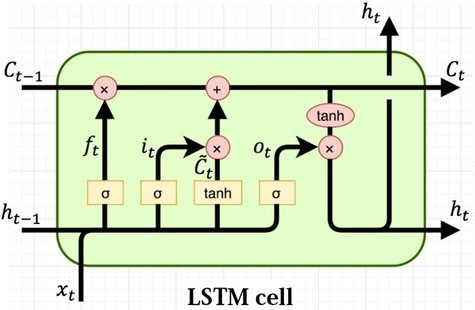
\includegraphics[width=0.5\linewidth]{LSTM.jpeg}
\end{center}

\textbf{Example}
Depending on the weights, the input $\mathbf{x}_{(t)}$ could have only a small effect on $y_{(t)}$ but a large effect on the long term memory $C_{(t)}$ and thus also on later outputs $y_{(t+n)} (n>1)$.